\pagebreak

\section{Modèle de Porter}

\begin{figure}[H]
	\begin{center}
		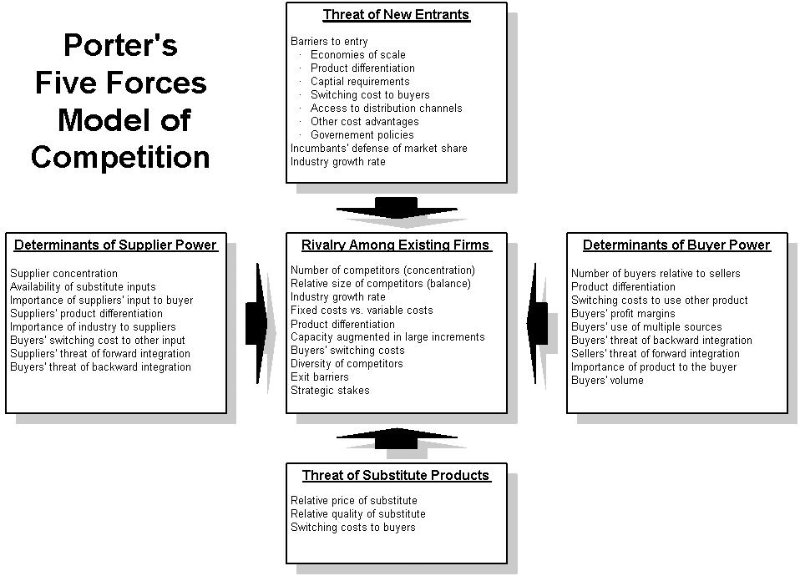
\includegraphics[scale=0.48]{images/porter/porter_1}
		\caption{Modèle de Porter}
		\label{inclusion}
	\end{center}
\end{figure}

\section{Analyse de marché}

\subsection{Définition du marché}

Cette étude porte sur les sociétés de Fret Aérien Civil Traditionnelles (FACT) qui gèrent leur propre flotte aérienne pour le transport de biens. Ce qui exclus le fret militaire ainsi que les logisticiens, entreprises de fret "virtuelles", qui font du point à point et louent des charters ou achètent des emplacements aux compagnies de fret traditionnlles. Les compagnies virtuelles constituent donc à la fois des clients pour le Fret Aérien Civil Traditionnel (FACT) qui permet à ces dernières d'optimiser le remplissage de leurs avions-cargo, mais aussi une forme de concurrence puisque le fret transporté au nom du logisticien est "perdu" pour tous les transporteurs classiques, y compris celui qui assure réellement le service. 

\subsection{Description des produits concernés}
Pour évaluer la concurrence, il convient d'étudier en premier lieu, le type de produits transportés. En effet, le pétrole ou le gaz, ne sont pas en général, transportés par avions ; sur ces matières premières, le fret aérien ne concurrence pas les secteurs maritimes, fluviaux, routiers ou par oléoduc/gazoduc. 

Le fret aérien, pour être compétitif, concerne donc les produits à haut rapport valeur sur poids ou à forte contrainte temporelle :

\begin{itemize}
	\item Electronique,
	\item Produits périssables : fleurs, fruits, 
	\item Animaux,
	\item Produits urgents ou à finalités humanitaires.
\end{itemize}



\subsection{Problème de la non  bi-directionnalité}
Pb pour rentabiliser le retour contrairement au transport passager.
solution : route multisecteur avec passage par plusieurs aéroports
mais solution non viable pour les produits périssables.





\subsection{Typologie du mode de transport du fret}


\begin{enumerate}
	\item avions cargo dédiés
	\item transport en soute dans avions passagers
	\item avion cargo combinés i.e. avions configurés de manière permanente pour le transport de fret et de PAX.
	\item avions reconfigurable rapidement pour les deux types de transport
\end{enumerate}

type avions très variable

\begin{enumerate}
	\item gros porteur B747-8F rayon d'action : 8000km 140 tonnes de fret
	\item avions spécialisés : Beluga AirBus A300 reconverti.
	\item petit porteur : twin turboprop Cessna super cargomaster 1700km 1.8 tonnes
\end{enumerate}